% asset_id: AS2ModellingInMechanicsTIKZ-003
\documentclass[tikz,border=8pt]{standalone}
\usepackage{amsmath}
\begin{document}
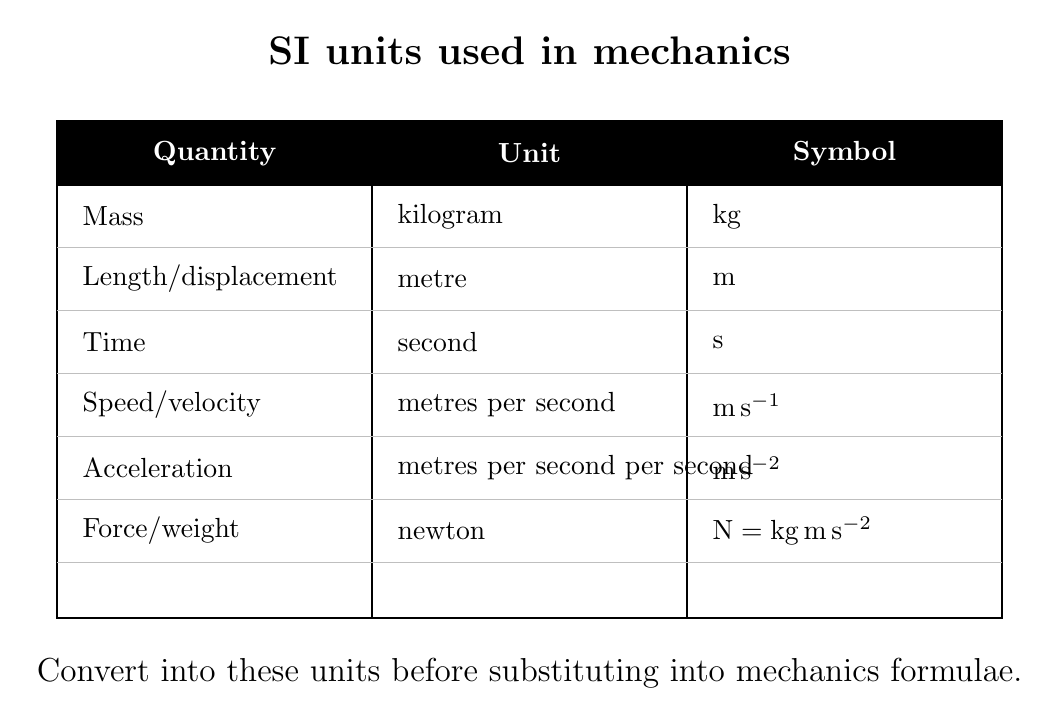
\begin{tikzpicture}
\node[font=\Large\bfseries] at (0,4.2) {SI units used in mechanics};
\draw[thick] (-6,3.3) rectangle (6,-3.0);\draw[thick, fill=black] (-6,3.3) rectangle (6,2.5);
\node[text=white, font=\bfseries] at (-4,2.9) {Quantity};\node[text=white, font=\bfseries] at (0,2.9) {Unit};\node[text=white, font=\bfseries] at (4,2.9) {Symbol};
\draw[thick] (-2,3.3) -- (-2,-3.0);\draw[thick] (2,3.3) -- (2,-3.0);
\foreach \y in {1.7,0.9,0.1,-0.7,-1.5,-2.3} {\draw[gray!50] (-6,\y) -- (6,\y);}
\node[anchor=west] at (-5.8,2.1) {Mass};\node[anchor=west] at (-1.8,2.1) {kilogram};\node[anchor=west] at (2.2,2.1) {$\mathrm{kg}$};
\node[anchor=west] at (-5.8,1.3) {Length/displacement};\node[anchor=west] at (-1.8,1.3) {metre};\node[anchor=west] at (2.2,1.3) {$\mathrm{m}$};
\node[anchor=west] at (-5.8,0.5) {Time};\node[anchor=west] at (-1.8,0.5) {second};\node[anchor=west] at (2.2,0.5) {$\mathrm{s}$};
\node[anchor=west] at (-5.8,-0.3) {Speed/velocity};\node[anchor=west] at (-1.8,-0.3) {metres per second};\node[anchor=west] at (2.2,-0.3) {$\mathrm{m\,s^{-1}}$};
\node[anchor=west] at (-5.8,-1.1) {Acceleration};\node[anchor=west] at (-1.8,-1.1) {metres per second per second};\node[anchor=west] at (2.2,-1.1) {$\mathrm{m\,s^{-2}}$};
\node[anchor=west] at (-5.8,-1.9) {Force/weight};\node[anchor=west] at (-1.8,-1.9) {newton};\node[anchor=west] at (2.2,-1.9) {$\mathrm{N=kg\,m\,s^{-2}}$};
\node[font=\large] at (0,-3.7) {Convert into these units before substituting into mechanics formulae.};
\end{tikzpicture}
\end{document}
